\documentclass{article}[18pt]
\ProvidesPackage{format}
%Page setup
\usepackage[utf8]{inputenc}
\usepackage[margin=0.7in]{geometry}
\usepackage{parselines} 
\usepackage[english]{babel}
\usepackage{fancyhdr}
\usepackage{titlesec}
\hyphenpenalty=10000

\pagestyle{fancy}
\fancyhf{}
\rhead{Sam Robbins}
\rfoot{Page \thepage}

%Characters
\usepackage{amsmath}
\usepackage{amssymb}
\usepackage{gensymb}
\newcommand{\R}{\mathbb{R}}

%Diagrams
\usepackage{pgfplots}
\usepackage{graphicx}
\usepackage{tabularx}
\usepackage{relsize}
\pgfplotsset{width=10cm,compat=1.9}
\usepackage{float}

%Length Setting
\titlespacing\section{0pt}{14pt plus 4pt minus 2pt}{0pt plus 2pt minus 2pt}
\newlength\tindent
\setlength{\tindent}{\parindent}
\setlength{\parindent}{0pt}
\renewcommand{\indent}{\hspace*{\tindent}}

%Programming Font
\usepackage{courier}
\usepackage{listings}
\usepackage{pxfonts}

%Lists
\usepackage{enumerate}
\usepackage{enumitem}

% Networks Macro
\usepackage{tikz}


% Commands for files converted using pandoc
\providecommand{\tightlist}{%
	\setlength{\itemsep}{0pt}\setlength{\parskip}{0pt}}
\usepackage{hyperref}

% Get nice commands for floor and ceil
\usepackage{mathtools}
\DeclarePairedDelimiter{\ceil}{\lceil}{\rceil}
\DeclarePairedDelimiter{\floor}{\lfloor}{\rfloor}

% Allow itemize to go up to 20 levels deep (just change the number if you need more you madman)
\usepackage{enumitem}
\setlistdepth{20}
\renewlist{itemize}{itemize}{20}

% initially, use dots for all levels
\setlist[itemize]{label=$\cdot$}

% customize the first 3 levels
\setlist[itemize,1]{label=\textbullet}
\setlist[itemize,2]{label=--}
\setlist[itemize,3]{label=*}

% Definition and Important Stuff
% Important stuff
\usepackage[framemethod=TikZ]{mdframed}

\newcounter{theo}[section]\setcounter{theo}{0}
\renewcommand{\thetheo}{\arabic{section}.\arabic{theo}}
\newenvironment{important}[1][]{%
	\refstepcounter{theo}%
	\ifstrempty{#1}%
	{\mdfsetup{%
			frametitle={%
				\tikz[baseline=(current bounding box.east),outer sep=0pt]
				\node[anchor=east,rectangle,fill=red!50]
				{\strut Important};}}
	}%
	{\mdfsetup{%
			frametitle={%
				\tikz[baseline=(current bounding box.east),outer sep=0pt]
				\node[anchor=east,rectangle,fill=red!50]
				{\strut Important:~#1};}}%
	}%
	\mdfsetup{innertopmargin=10pt,linecolor=red!50,%
		linewidth=2pt,topline=true,%
		frametitleaboveskip=\dimexpr-\ht\strutbox\relax
	}
	\begin{mdframed}[]\relax%
		\centering
		}{\end{mdframed}}



\newcounter{lem}[section]\setcounter{lem}{0}
\renewcommand{\thelem}{\arabic{section}.\arabic{lem}}
\newenvironment{defin}[1][]{%
	\refstepcounter{lem}%
	\ifstrempty{#1}%
	{\mdfsetup{%
			frametitle={%
				\tikz[baseline=(current bounding box.east),outer sep=0pt]
				\node[anchor=east,rectangle,fill=blue!20]
				{\strut Definition};}}
	}%
	{\mdfsetup{%
			frametitle={%
				\tikz[baseline=(current bounding box.east),outer sep=0pt]
				\node[anchor=east,rectangle,fill=blue!20]
				{\strut Definition:~#1};}}%
	}%
	\mdfsetup{innertopmargin=10pt,linecolor=blue!20,%
		linewidth=2pt,topline=true,%
		frametitleaboveskip=\dimexpr-\ht\strutbox\relax
	}
	\begin{mdframed}[]\relax%
		\centering
		}{\end{mdframed}}
\lhead{CSys  - Operating Systems}


\begin{document}
\begin{center}
\underline{\huge Mass Storage Systems - And Dinosaurs, boi}
\end{center}
\section{Overview of Mass Storage Structure}
\begin{itemize}
	\item Magnetic disks provide bulk of secondary storage of modern computers
	\begin{itemize}
		\item Transfer rate is the rate at which data flows between the drive and the computer
		\item Positioning time (random access time) is time to move disk arm to desired cylinder (seek time) and time for desired sector to rotate under the disk head (rotational latency)
		\item Head crash results from a disk head making contact with the disk surface
	\end{itemize}
	\item Disks can be removable
	\item Drive attached to computer via I/O bus
	\begin{itemize}
		\item Busses vary
		\item Host controller in computer uses bus to talk to disk controller built into drive or storage array
	\end{itemize} 
\end{itemize}
\section{Moving head disk mechanism}
\begin{center}
	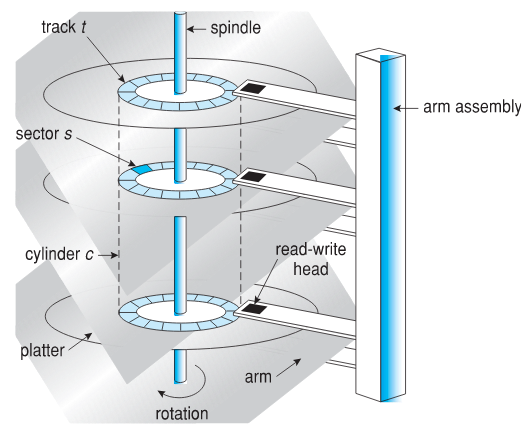
\includegraphics[scale=0.7]{mechanism}
\end{center}
\section{Hard Disk Performance}
\begin{itemize}
	\item Access Latency = Average access time = Average seek time + average latency
	\item Average I/O time = average access time + (amount to transfer/transfer rate)+controller overhead
\end{itemize}
\section{Solid State Disks}
\begin{itemize}
	\item Non-volatile memory used like a hard drive
	\item Can be more reliable than HDDs
	\item More expensive per MB
	\item Maybe have a shorter life span
	\item Less capacity
	\item But much faster
	\item Busses can be too slow $\rightarrow$ connect directly to PCI for example
	\item No moving parts, so no seek time or rotational latency 
\end{itemize}
\section{Magnetic Tape}
\begin{itemize}
	\item Relatively permanent and holds large quantities of data
	\item Access time slow
	\item Random access ~ 1000 times slower than disk
	\item Mainly used for backup, storage of infrequently used data, transfer medium between systems
	\item Kept in spool and wound or rewound past read-write head
\end{itemize}
\section{Disk Structure}
\begin{itemize}
	\item Disk drives are addressed as large 1-dimensional arrays of logical blocks, where the logical block is the smallest unit of transfer
	\item The 1 dimensional array of logical blocks is mapped into the sectors of the disk sequentially
	\begin{itemize}
		\item Sector 0 is the first sector of the first track on the outermost sylinder
		\item Mapping proceeds in order though that track, then the rest of the tracks in that cylinder, and then through the rest of the cylinders from outermost to innermost
	\end{itemize}
	\item Logical to physical addresses should be easy
	\begin{itemize}
		\item Except for bad sectors
		\item Non constant number of sectors per track via constant angular velocity
	\end{itemize}
\end{itemize}
\section{Storage Array}
\begin{itemize}
	\item Can just attach disks,or arrays of disks
	\item Storage array has controller(s), provides features to attached host(s)
	\begin{itemize}
		\item Ports to connect hosts to array
		\item Memory, controlling software
		\item A few to thousands of disks
		\item RAID, hot spares, hot swap
		\item Shared storage $\rightarrow$ more efficiency
		\item Features found in some file systems
		\begin{itemize}
			\item Snapshots, clones, thin provisioning, replication, de duplication etc
		\end{itemize}
	\end{itemize}
\end{itemize}
\section{Disk Scheduling}
\begin{itemize}
	\item The operating system is responsible for using hardware efficiently - for the disk drives, this means having a fast access time and disk bandwidth
	\item Minimize seek time
	\item Seek time $\approx$ seek distance
	\item Disk \textbf{bandwidth} is the total number of bytes transferred, divided by the total time between the first request for service and the completion of the last transfer
	\item There are many sources of disk I/O request
	\begin{itemize}
		\item OS
		\item System processes
		\item Users processes
	\end{itemize}
	\item I/O request includes input or output mode, disk address, memory address, number of sectors to transfer
	\item OS maintains queue of request, per disk or device
	\item Idle disk can immediately work on I/O request, busy disk means work must queue
	\begin{itemize}
		\item Optimisation algorithms only make sense when a queue exists
	\end{itemize}
	\item Note that drive controllers have small buffers and can manage a queue of I/O requests (of varying "depth")
	\item Several algorithms exist to schedule the servicing of disk I/O requests
	\item The analysis is true for one or many platters
	\item We illustrate scheduling algorithms with a request queue (0-199)
	$$98,183,37,122,14,124,65,67$$
	Head pointer 53
\end{itemize}
\section{FCFS}
Illustration shows total head movement of 640 cylinders\\
queue =98,183,37,122,14,124,65,67\\
Heads starts at 53
\begin{center}
	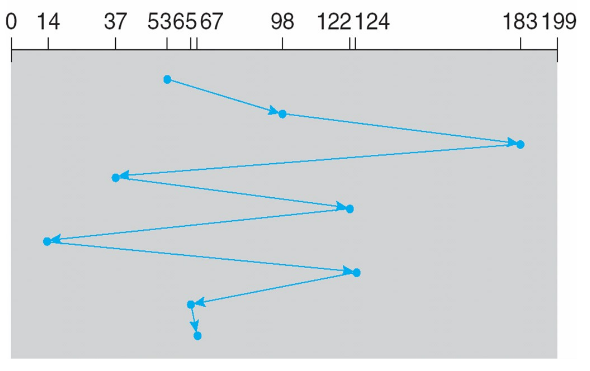
\includegraphics[scale=0.7]{FCFS}
\end{center}
\section{SSTF}
\begin{itemize}
	\item Shortest Seek time first selects the request with the minimum seek time from the current head position
	\item SSTF scheduling is a form of SJF scheduling; may cause starvation of some requests
	\item Illustration shows total head movement of 236 cylinders
\end{itemize}
\begin{center}
	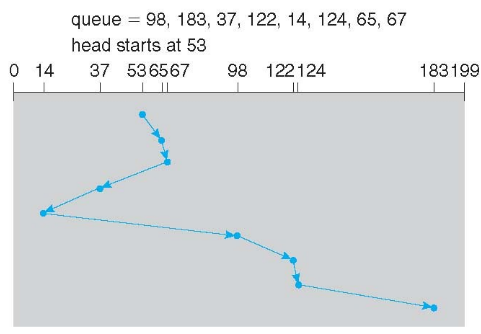
\includegraphics[scale=0.7]{SSTF}
\end{center}
\section{SCAN}
\begin{itemize}
	\item The disk arm starts at one end of the disk, and moves towards the other end, servicing requests until it gets to the other end of the disk, where the head movement is reversed and servicing continues
	\item SCAN algorithm, sometimes called the elevator algorithm
	\item Illustration shows total head movement of 236 cylinders
	\item But note that if the requests are uniformly dense, largest density at other end of disk and those wait the longest
\end{itemize}
\begin{center}
	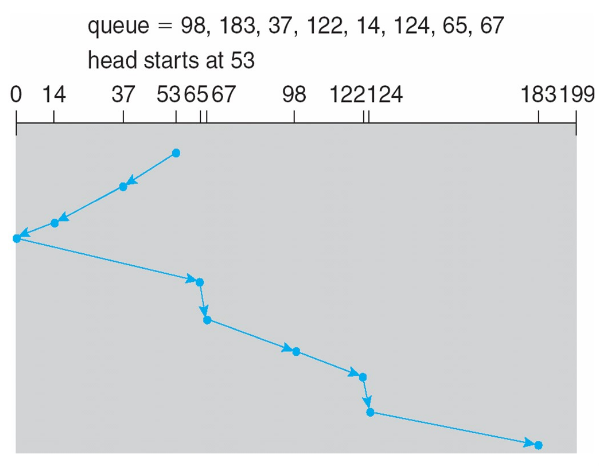
\includegraphics[scale=0.7]{SCAN}
\end{center}
\section{C-SCAN}
\begin{itemize}
	\item Provides a more uniform wait time than SCAN
	\item The head moves from one end of the disk to the other, servicing requests as it goes
	\begin{itemize}
		\item When it reaches the other end, however, it immediately returns to the beginning of the disk, without servicing any requests on the return trip
	\end{itemize}
	\item Treats the cylinders as a circular list that wraps around from the last cylinder to the first one
\end{itemize}
\begin{center}
	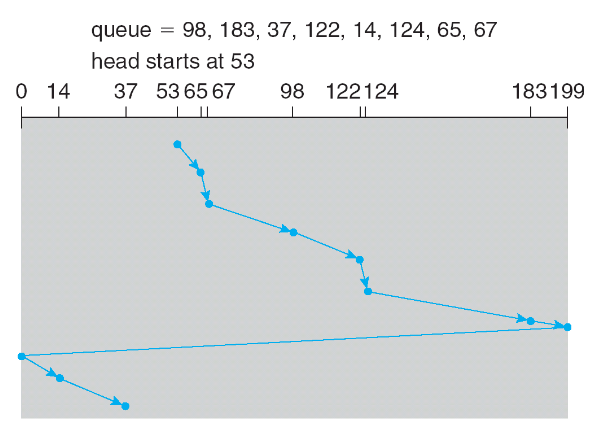
\includegraphics[scale=0.7]{C-Scan}
\end{center}
\section{C-LOOK}
\begin{itemize}
	\item LOOK a version of SCAN, C-LOOK a version of C-SCAN
	\item Arm only goes as far as the last request in each direction, then reverses direction immediately, without first going all the way to the end of the disk
\end{itemize}
\begin{center}
	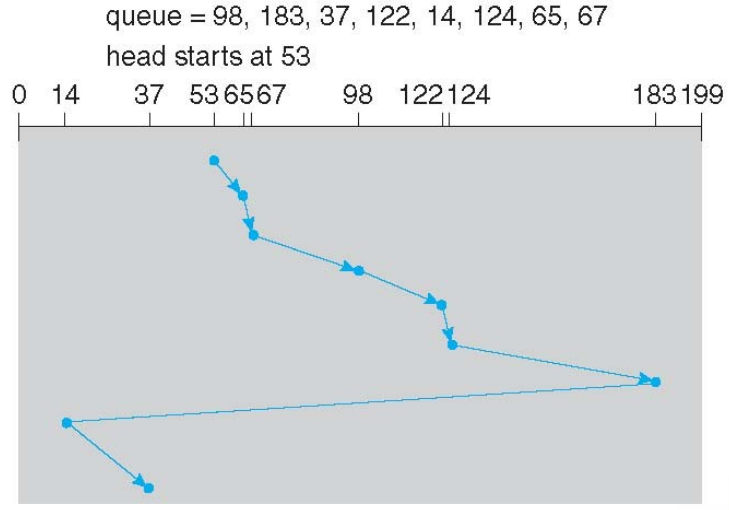
\includegraphics[scale=0.7]{C-LOOK}
\end{center}
\section{Selecting a Disk-Scheduling Algorithm}
\begin{itemize}
	\item SSTF is common and has natural appeal
	\item SCAN and C-SCAN perform better for systems that place a heavy load on the disk as there is less starvation
	\item Performance depends on the number and types of requests
	\item Requests for disk service can be influenced by the file-allocation method and metadata layout
	\item The disk-scheduling algorithm should be written as a separate module of the operating system, allowing it to be replaced with a different algorithm if necessary
	\item Either SSTF or LOOK is a reasonable choice for the default algorithm
	\item Rotational latency is difficult for the OS to calculate
\end{itemize}
\section{Disk Management}
\begin{itemize}
	\item Low level formatting, or physical formatting - dividing a disk into sectors that the disk controller can read and write
	\begin{itemize}
		\item Each sector can hold header information, plus data, plus error correction code
		\item Usually 512 bytes of data but can be selectable
	\end{itemize}
	\item To use a disk to hold files, the operating system still needs to record its own data structures on the disk
	\begin{itemize}
		\item Partition the disk into one or more groups of cylinders, each treated as a logical disk
		\item Logical formatting or "making a file system"
		\item To increase efficiency most file systems group blocks into clusters
		\begin{itemize}
			\item Disk I/O done in blocks
			\item File I/O done in clusters
		\end{itemize}
	\end{itemize}
	\item Raw disk access for apps that want to do their own block management, keep OS out of the way (databases for example)
	\item Boot block initialises system
	\begin{itemize}
		\item The bootstrap is stored in ROM
		\item Bootstrap loader program stored in boot blocks of boot partition
	\end{itemize}
	\item Methods such as sector sparing used to handle bad blocks
\end{itemize}
\section{Swap-Space Management}
\begin{itemize}
	\item Swap-space  - Virtual memory uses disk space as an extension of main memory, this is less common now due to memory capacity increases
	\item Swap-space can be carved out of the normal file system, or, more commonly, it can be in a separate disk partition (raw)
	\item Swap-Space management
	\begin{itemize}
		\item 4.3BSD allocates swap space when process starts; holds text segment (the program) and data segment
		\item Kernel uses swap maps to track swap space use
		\item Solaris 2 allocates swap space only when a dirty page is forced out of physical memory, not when the virtual memory page is first creates
		\begin{itemize}
			\item File data written to swap space until write to file system requested
			\item Other dirty pages go to swap space due to no other home
			\item Text segment pages thrown out and reread from the file system as needed
		\end{itemize} 
	\end{itemize}
	\item What if a system runs out of swap space?
	\item Some systems allow multiple swap spaces
\end{itemize}
\section{RAID Structure}
\begin{itemize}
	\item RAID - Redundant array of inexpensive disks
	\begin{itemize}
		\item Multiple disk drives provides reliability by redundancy
	\end{itemize}
	\item Increases mean time to failure
	\item Mean time to repair - exposure time when another failure could cause data loss
	\item If mirrored disks fail independently, consider disk with 1300,000 mean time to failure and a 10 hour mean time to repair
	$$\text{Mean time to data loss} 100,000^2/(2\times 10)=500\times 10^6 \text{hours}$$
	\item Frequently combined with NVRAM to improve write performance
	\item Several improvements in disk use techniques involve the use of multiple disks working cooperatively
	\item Disk striping uses a group of disks as one storage unit
	\item RAID is arranged into six different levels
	\item RAID schemes improve performance and improve the reliability of the storage system by storing redundant data
	\begin{itemize}
		\item Mirroring or shadowing (RAID 1) keeps a duplicate of each disk
		\item Stripped mirrors (RAID 1+0) or mirrored stripes (RAID 0+1) provides high performance and high reliability
		\item Block interleaved parity (RAID 4,5,6) uses much less redundancy
	\end{itemize}
	\item RAID within a storage array can still fail if the array fails, so automatic replication of the data between the arrays is common
	\item Frequently, a small number of hot-spare disks are left unallocated, automatically replacing a failed disk and having data rebuilt onto them
\end{itemize}
\section{RAID Levels}
\begin{center}
	\includegraphics[scale=0.7]{"Raid Levels"}
\end{center}
\section{RAID (0+1) and (1+0)}
\begin{center}
	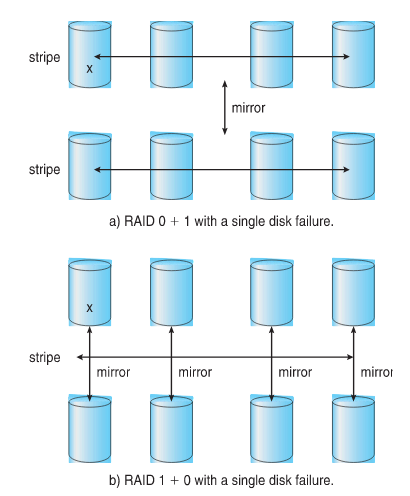
\includegraphics[scale=0.7]{RAID01}
\end{center}
\section{Other Features}
\begin{itemize}
	\item Regardless of where RAID implemented, other useful features can be added
	\item Snapshot is a view of the file system before a set of changes take place (i.e. at a point in time)
	\item Replication is automatic duplication of writes between separate sites
	\begin{itemize}
		\item For redundancy and disaster recovery
		\item Can be synchronous or asynchronous
	\end{itemize}
	\item Hot spare disk is unused, automatically used by RAID production is a disk fails to replace the failed disk and rebuild the RAID set if possible, decreasing mean time to repair
\end{itemize}
\section{Stable - Storage Implementation}
\begin{itemize}
	\item Write-ahead log scheme requires stable storage
	\item Stable storage means data is never lost (due to failure,etc)
	\item To implement stable storage:
	\begin{itemize}
		\item Replicate information on more than one nonvolatile storage media with independent failure models
		\item Update information in a controlled manner to ensure that we can recover the stable data after any failure during data transfer or recovery
	\end{itemize}
	\item Disk write has 1 of 3 outcomes
	\begin{enumerate}
		\item Successful completion - The data were written correctly on disk
		\item Partial failure - A failure occurred in the midst of a transfer, so only some of the sectors were written with the new data, and the sector being written during the failure may have been corrupted
		\item Total Failure - The failure occurred before the disk write started, so the previous data values on the disk remain intact
	\end{enumerate}
	\item If failure occurs during block write, recovery procedure restores block to a consistent state
	\begin{itemize}
		\item System maintains 2 physical blocks per logical block and does the following:
		\begin{enumerate}
			\item Write to 1st physical
			\item When successful, write to 2nd physical
			\item Declare complete only after second write completes successfully
		\end{enumerate}
		Systems frequently use NVRAM and one physical to accelerate
	\end{itemize}
\end{itemize}
\end{document}